\begin{tikzpicture}[scale = 1.25]

    \draw(0.5,0) rectangle (1.5,1.25)node[midway, rotate = 90]
    {\footnotesize \Blue{données}$_{\bm{1}}$};
    
    \draw[fill = lightgray!50!white](0,0) rectangle (0.5,1.25) node[midway, rotate = 90]
    {\footnotesize \Orange{pilotes}$_{\bm{1}}$};

    \draw[fill = lightgray!50!white](1.5,0) rectangle (2,1.25) node[midway, rotate = 90]
    {\footnotesize \Orange{pilotes}$_{\bm{2}}$};
    
    \draw(2,0) rectangle (3,1.25)node[midway, rotate = 90]
    {\footnotesize \Blue{données}$_{\bm{2}}$};

    \draw[dashed] (3,0) --++ (0.5,0);
    \draw[dashed] (3,1.25) --++ (0.5,0);

    \draw [fill = lightgray!50!white](-1.5,-1.5) rectangle(2,-0.5) node[midway]
    {$\cdots$};

    \draw [fill = lightgray!50!white](0.25,-2) node{\footnotesize 
    $\phi_{\Orange{p},\bm{1}} = 
    	\braket{\{\phi_{\Orange{p},\bm{1}\bullet}\}_\bullet}$};

    \draw [fill = lightgray!50!white] (-1.5,-1.5) rectangle(-0.75,-0.5) 
    node[midway, rotate = 90]{\footnotesize 
    $\substack{\Orange{p}_{\bm{1},1}\\ \equiv\phi_{\Orange{p}:\bm{1},1}}$};

	\draw [fill = lightgray!50!white] (1.25,-1.5) rectangle(2,-0.5) 
    node[midway, rotate = 90] {\footnotesize
    $\substack{\Orange{p}_{\bm{1},n_{\Orange{p}}}\\ 
    				\equiv\phi_{\Orange{p}:\bm{1},n_{\Orange{p}}}}$};

    \draw[dashed] (0,0) -- (-1.5,-0.5) --++ (3.5,0) -- (0.5,0);
    \draw (0,-1.5) node{};
    
%    \draw[color = white] (0,-2) rectangle (2,-3);
\end{tikzpicture}
